\documentclass[aspectratio=169]{beamer}

\usepackage[british]{babel}
\usepackage{lipsum}
\usepackage[T1]{fontenc}
\usepackage[utf8]{inputenc}
\usepackage{lmodern}
\usepackage{microtype}
\usepackage{ragged2e}
\usepackage{multicol}
\usepackage{paralist}
\usepackage{ulem}
\usepackage{blindtext}
%Bibliography
\usepackage[backend=biber, style = authoryear, sorting=nyt]{biblatex}
    \bibliography{references.bib}

\renewbibmacro*{cite}{%
  \iffieldundef{shorthand}
    {\ifthenelse{\ifnameundef{labelname}\OR\iffieldundef{labelyear}}
       {\usebibmacro{cite:label}%
        \setunit{\printdelim{nonameyeardelim}}}
       {\printnames{labelname}%
        \setunit{\printdelim{nameyeardelim}}}%
     \usebibmacro{cite:labeldate+extradate}%
     \setunit{\addcomma\space}%
     \usebibmacro{journal}
     \setunit{\addcomma\space}%
     \usebibmacro{title}}
    {\usebibmacro{cite:shorthand}}}

%Graphikeinbindungen
\usepackage{graphicx}
%\usepackage{sidecap}  
\usepackage{pgfplots}
    \pgfplotsset{compat = 1.15}
\usepackage{tikz}
    \usetikzlibrary{calc,quotes,arrows.meta,automata}
    \usetikzlibrary{overlay-beamer-styles}
\usepackage{tikz-dimline}
\usepackage[compat=1.1.0]{tikz-feynman}
%Farbeinstellungen für Hyperlinks und Pythoncode
\usepackage{xcolor}
    \definecolor{myred}  {HTML}{A3061E}
    \definecolor{myblue} {RGB} {0,63,119}
    \definecolor{myyellow} {cmy} {0,0.263,0.741}
    \definecolor{mygreen} {HTML}{0B6E4F}
    \colorlet{myorange} {myyellow!60!myred}
    \colorlet{myviolett} {myred!50!myblue!80}
%für Python code
\usepackage{listings}
	\lstdefinestyle{python}{
	language         = Python                   ,
	basicstyle       = \ttfamily                ,
	keywordstyle     = \color{myred}            ,
	identifierstyle  = \color{myblue}           ,
	stringstyle      = \color{mygreen}          ,
	commentstyle     = \color{black!50}         ,
	numberstyle      = \color{black!50}\tiny    ,
	numbers          = left                     ,
	belowcaptionskip = \baselineskip            ,
	}
%
\usepackage{caption}
    \captionsetup{%
        font=small,%
        format=plain,%
        labelfont=bf,%
        labelsep=colon,%
        margin=10pt,%
        textfont=sl,%
        singlelinecheck=true%
    }
%Gegen Widowline
\usepackage[defaultlines=2,all]{nowidow}
%Mathe-. und Physikdinge
\usepackage{amssymb, amsmath, amsfonts, amsthm, mathtools, nicefrac, bm, dsfont, upgreek}
\usepackage{mathrsfs}
\usepackage{tensor}
\usepackage{fixmath}
    \usefonttheme[onlymath]{serif}
\usepackage{physics,braket,siunitx}
\usepackage{csquotes}
\usepackage{hyperref}
    \renewcommand{\thefootnote}{\roman{footnote}}
%
\renewcommand{\vec}[1]{\bm{#1}}
\newcommand{\mat}[1]{\vphantom{\uuline{#1}}\smash{\uuline{\mkern-1mu \vphantom{\underline{#1}}#1\mkern-1mu}\mkern2mu}}
\newcommand{\uvec}[1]{\vphantom{\underline{#1}}\smash{\underline{\mkern-1mu #1\mkern-1mu}\mkern2mu}}


%\usepackage{appendixnumberbeamer}

\newcommand{\TaS}{TaS\textsubscript{2}\xspace}
\newcommand{\QE}{\textsc{Quantum} ESPRESSO\xspace}

\title[Bachelor's Colloquium]{Optimization of the Quantum Espresso Density Functional Theory Code for parallel execution on the PHYSnet-Cluster}
\author{Tjark Sievers}
\date{13th July 2022}
\institute[I. ITP -- AG Computational Condensed Matter Theory]{I. Institute of Theoretical Physics}

\usetheme{CCMT}


\begin{document}

{
\setbeamertemplate{footline}{\empty}
\begin{frame}
	\titlepage
\end{frame}
}
\addtocounter{framenumber}{-1}

\begin{frame}
	\frametitle{Motivation}

	\begin{itemize}
		\item Computing resources are limited, both in time and memory available
		\item This means: work has to be distributed efficiently among multiple processors
		\item Codes like \QE offer capabilities to tune how exactly the workload is distributed
		%\item Some problems need ideal parallelization so they can be solved on todays computer systems 
	\end{itemize}

	\vspace{10pt}

	\pause

	I aim to answer some questions:

	\begin{itemize}
		\item How big is the effect of good/bad parallelization?
		\item How does hardware topology play into it? (PHYSnet: 20 cores per node)
		\item How can one find good parallelization parameters?
		%\item \ldots
	\end{itemize}
\end{frame}



\begin{frame}[t]
	\frametitle{Speedup}

	\begin{columns}
		\begin{column}[T]{0.48\textwidth}
			How much faster can a problem be solved with \(N\) processors instead of one?
			
			\begin{equation*}
				S \coloneqq \frac{T_1}{T_N}
			\end{equation*}

			with serial runtime \(T_1\), runtime on \(N\) cores \(T_N\)
		\end{column}
		\begin{column}[T]{0.48\textwidth}
			\emph{Ideal case}: every processor needs the same time
			\begin{align*}
				T_N = \frac{T_1}{N}
				\implies S = \frac{T_1}{\frac{T_1}{N}} = N
			\end{align*}
		\end{column}
	\end{columns}
\end{frame}

\begin{frame}
	\frametitle{Amdahl's Law}
	
	\begin{columns}
		\begin{column}{0.48\textwidth}
			In reality: several factors limiting parallelization: communication between processors, startup time, algorithmic limitations

			\vspace{10pt}
			\pause

			Simple model given by \emph{Amdahl's law}
			\begin{equation*}
				S = \frac{T_1}{T_N} = \frac{1}{s + \frac{1 - s}{N}}
			\end{equation*}
			with \(s\) the part of the calculation which cannot be perfectly parallelized
		\end{column}

		\begin{column}{0.48\textwidth}
			\pause
			\includegraphics[width=0.9\textwidth]{figs/amdahl.pdf}
			\begin{itemize}
				\item upper bound for speedup given by \(\nicefrac{1}{s}\)
				\item smaller \(s\): closer to \(S = N\) for more processors
			\end{itemize}
			
		\end{column}
	\end{columns}
\end{frame}

\begin{frame}
	\frametitle{Solving the Kohn-Sham equations}

	\begin{columns}
	\begin{column}{0.5\textwidth}
	\centering
	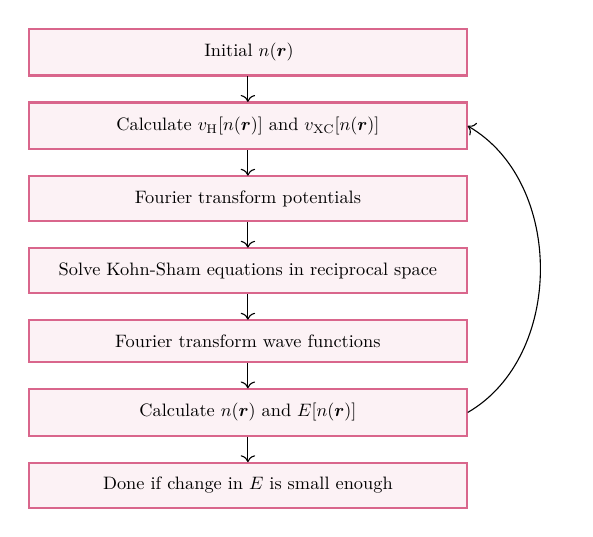
\begin{tikzpicture}[
		scale=0.65,transform shape, squarednode/.style={rectangle, draw=purple!60, fill=purple!5, thick, minimum size=5mm, text centered, text width=8cm,},
		node distance=0.5cm]
		\tikzset{every node/.style={inner sep=8pt}}
		%Nodes
		\node[squarednode]      (init)          {Initial \(n(\vb*{r})\)};
		\node[squarednode]      (step_1)    [below= of init]  {Calculate \(v_{\mathrm{H}} [n(\vb*{r})]\) and \(v_{\mathrm{XC}} [n(\vb*{r})]\)};
		\node[squarednode]      (step_2)    [below= of step_1]      {Fourier transform potentials};
		\node[squarednode]      (step_3)    [below= of step_2]      {Solve Kohn-Sham equations in reciprocal space};
		\node[squarednode]      (step_4)    [below= of step_3]      {Fourier transform wave functions};
		\node[squarednode]      (step_5)    [below= of step_4]      {Calculate \(n(\vb*{r})\) and \(E [n(\vb*{r})]\)};
		\node[squarednode]      (done)      [below= of step_5]      {Done if change in \(E\) is small enough};
		
		%Lines
		\draw[->] (init.south) -- (step_1.north);
		\draw[->] (step_1.south) -- (step_2.north);
		\draw[->] (step_2.south) -- (step_3.north);
		\draw[->] (step_3.south) -- (step_4.north);
		\draw[->] (step_4.south) -- (step_5.north);
		\draw[->] (step_5.east) to [out=30,in=-30] (step_1.east);
		\draw[->] (step_5.south) -- (done.north);
	\end{tikzpicture}
	\end{column}

	\begin{column}{0.5\textwidth}
		Basis set for periodic systems: plane waves
		\begin{equation*}
			\psi_{n \vb*{k}} (\vb*{r}) = \frac{1}{\sqrt{V}} \sum_{\vb*{G}} e^{i (\vb*{k} + \vb*{G}) \vb*{r}}
		\end{equation*}	

		%\vspace{10pt}

		Multiple ways to parallelize:

		\begin{itemize}
			\item distributing grids in real/reciprocal space (\emph{R/G parallelization})
			\item solve Kohn-Sham equations for different \(k\)-points separately (\emph{\(k\)-point parallelization})
		\end{itemize}
		
	\end{column}

	\end{columns}
\end{frame}

%\begin{frame}
%	\frametitle{DFPT calculations}
%
%	Phonon calculations are also possible within the framework of DFT

%	\vspace{10pt}

%	Task is again to solve a set of equations self-consistently, similar to the Kohn-Sham equations

%	Parallelization possibilities:
%		\begin{itemize}
%			\item Distributing grids in real/reciprocal space (enabled by default)
%			\item \(k\)-points parallelization
%			\item Split up calculations for different phonon wave vectors: \(q\)-point parallelization
%		\end{itemize}
%
%\end{frame}


\begin{frame}
	\frametitle{Parallelization parameters}

	\QE has the argument \texttt{nk}: determines number of processors pools the available processors are split into (for \(k\)-point parallelization)

	\(\leadsto\) different partition of the processors, depending on the total number of processors

	\begin{columns}
		\begin{column}{0.5\textwidth}
			\pause[2]\begin{center}
				no \(k\) point parallelization

				\includegraphics[width=0.3\textwidth]{figs/np16_no_kpoint.pdf}
			\end{center}

			\pause[3]\begin{center}
			\includegraphics[width=0.15\textwidth]{figs/np4_no_kpoint.pdf}			
			\end{center}
		\end{column}

		\begin{column}{0.5\textwidth}
			\pause[2]\begin{center}
				\texttt{nk 4}

				\centering
				\includegraphics[width=0.3\textwidth]{figs/np16_nk_4.pdf}			
			\end{center}

			\pause[3]\begin{center}
				\includegraphics[width=0.15\textwidth]{figs/np4_nk_4.pdf}			
			\end{center}
		\end{column}
	\end{columns}
	
	\vspace{8pt}

	\pause

	\(\leadsto\) use size of the resulting pools for comparison, not the parameter \texttt{nk}

\end{frame}


\begin{frame}
	\frametitle{Examined systems}

	\begin{columns}
		\begin{column}{0.5\textwidth}
			\centering
			\includegraphics[width=0.8\textwidth]{figs/symmetric.pdf}

			\begin{center}
				Monolayer Tantalum Disulfide (\TaS)

				light gray: symmetric structure

				dark gray/yellow: charge density wave phase
			\end{center}
			 %(\TaS) in a \(3\times 3\) charge density wave
		\end{column}

		\begin{column}{0.5\textwidth}
			\centering
			\includegraphics[width=0.8\textwidth]{figs/Silicon.png}

			\begin{center}
				Silicon
			\end{center}
		\end{column}
	\end{columns}	

\end{frame}


% pwscf

\begin{frame}
	\frametitle{Electronic structure\\ No \(k\)-point parallelization}
	
	\begin{columns}
		\begin{column}{0.5\textwidth}
			\includegraphics[width=0.9\textwidth]{figs/TaS2_ompi_bench_nprocs_speedup.pdf}
			\begin{itemize}
				\item OpenMPI/gcc compilers
				\item decline in speedup after 20 processors
			\end{itemize}
		\end{column}

		\begin{column}{0.5\textwidth}
				\includegraphics[width=0.9\textwidth]{figs/TaS2_intel_bench_nprocs_speedup.pdf}
			\begin{itemize}
				\item Intel compilers
				\item ideal speedup for up to 40 processors
			\end{itemize}
		\end{column}
	\end{columns}
\end{frame}


\begin{frame}
	\frametitle{Electronic structure\\ \(k\)-point parallelization}
	
	\begin{columns}
		\begin{column}{0.5\textwidth}
			\begin{figure}
				\includegraphics[width=\textwidth]{figs/TaS2_intel_bench_nk_speedup.pdf}
			\end{figure}
		\end{column}

		\begin{column}{0.5\textwidth}
			\begin{itemize}
				\item pool size 36 scales best
				\item consistent with the results of the benchmark without \(k\)-point parallelization
			\end{itemize}
		\end{column}
	\end{columns}

\end{frame}

\begin{frame}
	\frametitle{Electronic structure\\ \(k\)-point parallelization}
	
	\begin{columns}
		\begin{column}{0.5\textwidth}
			\begin{figure}
				\includegraphics[width=\textwidth]{figs/TaS2_intel_bench_nk_speedup.pdf}
				\caption*{PHYSnet}
			\end{figure}
		\end{column}

		\begin{column}{0.5\textwidth}
			\begin{figure}
				\includegraphics[width=\textwidth]{figs/TaS2_hlrn_bench_nk_speedup.pdf}
				\caption*{HLRN}
			\end{figure}
		\end{column}
	\end{columns}

\end{frame}


%\begin{frame}
%	\frametitle{\(k\)-point parallelization}
	
%	\begin{columns}
%		\begin{column}{0.5\textwidth}
%			\begin{figure}
%				\includegraphics[width=\textwidth]{figs/TaS2_hlrn_bench_nk_speedup.pdf}
				%\caption*{HLRN}
			%\end{figure}
		%\end{column}
		%\begin{column}{0.5\textwidth}
			%\begin{itemize}
				%\item hardware topology is completely different: nodes have 96 cores each
				%\item pool size 36  still scales best
				%\item other pool sizes show a similar scaling as well
			%\end{itemize}	
		%\end{column}
	%\end{columns}

%\end{frame}

% Phonons

\begin{frame}
	\frametitle{Phonons\\ Preliminaries \& \(k\)-point parallelization}

	\begin{columns}
		\begin{column}{0.5\textwidth}
			%Some formula

			DFPT: again a set of equations to be solved self-consistently

			\vspace{10pt}

			Multiple ways to parallelize:

			\begin{itemize}
				\item \emph{R/G parallelization}
				\item \emph{\(k\)-point parallelization}
				\item separate calculations for different phonon wave vectors \(q\) (\emph{image parallelization})
			\end{itemize}
		\end{column}
		\pause
		\begin{column}{0.5\textwidth}
			Phonon calculations at \(q = 0\)

			Two pool sizes tested, both on 180 processors:
			\begin{itemize}
				\item pool size 18: \SI{3044}{\minute}
				\item pool size 36: \SI{2020}{\minute}
			\end{itemize}

			\vspace{10pt}

			Difference already after first phonon mode:
			\begin{itemize}
				\item pool size 18: \SI{2832.1}{\second}
				\item pool size 36: \SI{2183.3}{\second}
			\end{itemize}

			\(\leadsto\) optimal pool size translates over modules
		\end{column}
	\end{columns}
\end{frame}

%\begin{frame}
%	\frametitle{Image parallelization}
%
%	\begin{columns}
%		\begin{column}{0.5\textwidth}
%			\begin{figure}
%				\includegraphics[width=\textwidth]{figs/si_ph_poolsize_8_images_distribution.pdf}
%			\end{figure}
%		\end{column}
%
%		\begin{column}{0.5\textwidth}
%			\begin{itemize}
%				\item 
%			\end{itemize}
%		\end{column}
%	\end{columns}
%
%\end{frame}

\begin{frame}
	\frametitle{Phonon calculations\\ Image parallelization}

	\begin{columns}
		\begin{column}{0.5\textwidth}
			\begin{figure}
				\includegraphics[width=\textwidth]{figs/si_ph_poolsize_8_bench_ni_speedup.pdf}
			\end{figure}
		\end{column}

		\begin{column}{0.5\textwidth}
			\begin{itemize}
				\item benchmark run on bulk silicon
				\item for that system: pool size 8 performed best
				\item[\(\leadsto\)] benchmark with combinations of \texttt{ni} and \texttt{nk} with resulting pool size of 8
				\item linear scaling continues when using more images
			\end{itemize}
		\end{column}
	\end{columns}

\end{frame}


% Conclusion

\begin{frame}
	\frametitle{Conclusion}


	\begin{columns}
		\begin{column}{0.5\textwidth}
			\begin{itemize}
				\item goal of this thesis: examine how \QE calculations parallelize, measured by speedup
				\pause\item right choice of parallelization parameters has a significant impact on the runtime of calculations with \QE
				\pause\item good choice of parameters translates between the two modules examined and between different compute clusters
			\end{itemize}
		\end{column}
		\begin{column}{0.5\textwidth}
			\centering
			\pause[2]\includegraphics[height=0.5\textheight]{figs/TaS2_intel_bench_nk_speedup.pdf}
			\pause[2]\includegraphics[height=0.5\textheight]{figs/si_ph_poolsize_8_bench_ni_speedup.pdf}
		\end{column}
	\end{columns}

\end{frame}

% Folien für Rückfragen

%\appendix
\begin{frame}
	\centering
	{\huge Additional slides}
\end{frame}

%\begin{frame}
%	\frametitle{Factors limiting parallel execution}
%\end{frame}

\begin{frame}
	\frametitle{\(k\) point parallelization: Memory}

	Electronic structure calculations on \TaS, 180 processors

	\vspace{10pt}

	pool size 18:
	\begin{itemize}
		\item estimated max dynamical RAM per process > 178.04 MB
		\item estimated total dynamical RAM > 28.67 GB
	\end{itemize}

	pool size 36:
	\begin{itemize}
		\item estimated max dynamical RAM per process > 103.76 MB
		\item estimated total dynamical RAM > 17.07 GB
	\end{itemize}
\end{frame}

\begin{frame}
	\frametitle{Electronic structure calculations}

	\centering
	\includegraphics[width=0.6\textwidth]{figs/TaS2_intel_bench_nprocs_absolute.pdf}

\end{frame}

%\begin{frame}
%	\frametitle{Compilers?}

%	Intel

%	OpenMPI

%\end{frame}

\begin{frame}
	\frametitle{Amdahl's Law: limitations}

	\begin{itemize}
		\item no distinction between different limiting factors: e.g. communication limits parallelization with some dependence on \(N\)
		\item[\(\leadsto\)] serial part \(s\) gives no information about what could be improved
	\end{itemize}

\end{frame}

\end{document}
